%==========================================================
% Titel:    Formelsammlung-HSR
% Autor:    Adrian Freihofer
% Erstellt: 7.11.2001
% Ge�ndert:
%==========================================================

\chapter{Statik}  \index{Statik}


\section{Starre K�rper im Gleichgewicht}                        \index{Starre K�rper im Gleichgewicht}

\subsection{Gleichgewichtsbedingung starrer K�rper}             \index{Gleichgewichtsbedingung}
                                                                
\Hauptbox{
  \Bildbox{
 Ein K�r"-per ist dann im Gleich"-ge"-wicht, wenn kei"-ne re"-sul"-tie"-ren"-de Kraft auf ihn wirkt, d.h. die Summe der ihn an"-grei"-fen"-den Kr�fte ist null.
%  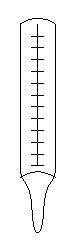
\includegraphics{Physik/Warmelehre/termometer.eps}
  }

  \Formelbox{
    Allgemein: \[ \sum_{i=1}^n \vec{F_i}=0 \mbox{\hspace{1cm}} \sum_{i=1}^n \vec{M_i}=0 \]  
   \small{ In Komponenten: \[ \sum_{i=1}^n \vec{F_{ix}}=0 \mbox{\hspace{1cm}} \sum_{i=1}^n \vec{M_{ix}}=0 \]  
    \[ \sum_{i=1}^n \vec{F_{iy}}=0 \mbox{\hspace{1cm}} \sum_{i=1}^n \vec{M_{iy}}=0 \]
    \[ \sum_{i=1}^n \vec{F_{iz}}=0 \mbox{\hspace{1cm}} \sum_{i=1}^n \vec{M_{iz}}=0 \]}
   }
  }
  {\Groessenbox{
     $ F$          & Kraft         & $ [N] $                 \\   
     $ M $         & Drahmoment    & $ [Nm]$ \\
}}

\subsection{Haftreibung}         \index{Haftreibung}

\Hauptbox{
  \Bildbox{
  \input{Physik/Statik/Haftreibung.pstex_t}
  }

  \Formelbox{
    \[ \vec{F_N} = \vec{F_G} \hspace{1cm} \vec{F_R} = \vec{F}  \]   
    \[ \vec{F_R} \le \vec{F_{Rmax}} \le \mu_H F_N\]  

   }
  }
  {\Groessenbox{ 
      $ F$          & Kraft           & $ [N] $                 \\   
      $ F_G$        & Gewichtskraft   & $ [N] $                 \\   
      $ F_N$        & Normalkraft     & $ [N] $                 \\ 
      $ F_R$        & Reibkraft       & $ [N] $                 \\     
      $ \mu_H$      & Haft"-rei"-bungs"-koef"-fi"-zient           & $ [1] $                 \\   
}}
\vfill

\subsection{Reaktionsprinzip}

\index{Reaktionsprinzip}

\Hauptbox{
  \Bildbox{
    Das Reaktionsprinzip gilt, wenn zwei K�rper Kr�fte auf einander aus�ben.
  }

  \Formelbox{
    \[ \vec{F_{BA}} = - \vec{F_{AB}} \]  

   }
  }
  {\Groessenbox{ 
      $ F_{AB}$        & Kraft von K�r"-per A    & $ [N] $                 \\   
      $ F_{BA}$        & Kraft von K�r"-per B    & $ [N] $                 \\   
}}


\subsection{Drehmoment}

\index{Drehmoment}
\index{Kr�ftepaar}

\subsubsection{Drehmoment eines Kr�ftepaars}

\Hauptbox{
  \Bildbox{
     \input{Physik/Statik/Drehmoment.pstex_t}
  }
  \Formelbox{
    \[ M = a F \]  
    $\vec M$ $\bot$ auf Ebene $\vec{r}$ , $\vec{F}$ : \[ M = F r \sin(\alpha)\]
   Drehmomente nicht in einer Ebene: \[ \vec{M} = \vec{r} \times \vec{F} \]  
    \footnotesize{Drehsinn im Gegenuhrzeigersinn: +}
   }
  }
  {\Groessenbox{ 
      $ M$        & Drehmoment    & $ [Nm] $                 \\   
      $ a$        & Abstand       & $ [m] $                 \\    
      $ F$        & Kraft         & $ [N] $                 \\    
      $ r$        & Radius        & $ [m] $                 \\   
}}

\subsubsection{Drehmoment einer Einzelkraft}

\index{Einzelkraft}

\Hauptbox{
  \Bildbox{
     \input{Physik/Statik/DrehmomentEinz.pstex_t}
  }

  \Formelbox{
    \[ M = a F \]  
    \[ \vec M = \vec r \times \vec F \]
   }
  }
  {\Groessenbox{ 
      $ M$        & Drehmoment    & $ [Nm] $                 \\   
      $ a$        & Abstand       & $ [m] $                 \\    
      $ F$        & Kraft         & $ [N] $                 \\    
      $ r$        & Radius        & $ [m] $                 \\   
}}
\vfill


\section{Schwerpunkt}

\index{Schwerpunkt}

\Hauptbox{
  \Bildbox{
     \input{Physik/Statik/Schwerpunkt.pstex_t}
  }

  \Formelbox{
    \[ x_s = \frac{\sum_i x_i m_i}{\sum_i m_i} \] 
    \[ y_s = \frac{\sum_i y_i m_i}{\sum_i m_i} \]  
    \[ z_s = \frac{\sum_i z_i m_i}{\sum_i m_i} \] 
    \scriptsize Schwerpunkt eines Halbkreises: \normalsize
    \[  x=0 \mbox{\hspace{1cm}} y = \frac{4r}{3 \pi} \]
   }
  }
  {\Groessenbox{ 
      $ x_s$, 
      $y_s$,  
      $z_s$      & Koor"-di"-na"-ten des Ge"-samt"-schwer"-punk"-tes    & $ [m] $     \\   
      $ x_i$, 
      $y_i$, 
      $z_i$      & Schwer"-punkts"-koor"-di"-na"-ten Teil"-k�r"-per i       & $ [m] $     \\    
      $ r$        & Radius        & $ [m] $                 \\   
}}

\section{Deformierung}

\index{Deformierung}

\subsection{Spannung}

\index{Spannung}

\Hauptbox{
  \Bildbox{
     \input{Physik/Statik/Spannung.pstex_t}
  }

  \Formelbox{
    \[ \sigma = \frac{F_\bot}{A} \] 
    \[ \tau = \frac{F_\parallel}{A} \]  
    \[ p = - \sigma \] 
    }
  }
  {\Groessenbox{ 
      $ \sigma $  & Zugspannung      & $ [\frac{N}{m^2}] $                 \\   
      $ \tau $    & Schubspan"-nung  & $ [\frac{N}{m^2}] $                 \\    
      $ p $       & Druck            & $ [\frac{N}{m^2}] $                 \\       
      $ A $       & Fl�che           & $ [m^2] $                 \\      
      $ F $       & Kraft            & $ [N] $                 \\      
}}




\subsection{Dehnung}
\index{Dehnung}

\Hauptbox{
  \Bildbox{
     \input{Physik/Statik/Dehnung.pstex_t}
  }

  \Formelbox{
    \[ \epsilon = \frac{\Delta l}{l} \]
    \[ \Delta l \sim \frac{l F}{A} \]
    \[ \epsilon = \frac{1}{E} \sigma = \frac{1}{E} \frac{F}{A} \]
    \vspace{0.3cm}
   }
  }
  {\Groessenbox{ 
      $ \epsilon $ & Dehnung                    & $ [ 1 ] $                 \\   
      $ A $        & Querschnitts"-fl�che       & $ [m^2] $                 \\    
      $ l $        & Balkenl�nge                & $ [m] $                 \\    
      $ F $        & Kraft                      & $ [N] $                 \\     
      $ E $        & Elastizit�ts"-modul        & $ [\frac{N}{m^2}] $                 \\   
      $\sigma$     & Zugspannung                & $ [\frac{N}{m^2}]$\\
}}
\vfill

\subsection{Querkontraktion}

\index{Querkontraktion}

\Hauptbox{
  \Bildbox{
     Die Querkontraktion entspricht dem D�nnenrwerden eines Materials bei Dehnung
  }
  \Formelbox{
    \[ \epsilon_q = \frac{\Delta d }{d} = \frac{-\mu \Delta l}{l}\]
    \[ \epsilon_q = - \mu \epsilon \]
    \vspace{1cm}
   }
  }
  {\Groessenbox{ 
      $ \epsilon_q $   & Querkon"-trak"-tion    & $ [ 1 ] $                 \\   
      $ \mu $          & Poissonzahl            & $ [ 1 ] $                 \\    
      $ d $            & Dicke Material         & $ [m] $                 \\    
      $ l $            & L�nge                  & $ [m] $                 \\   
}}



\subsection{Kompression}

\index{Kompression}

\Hauptbox{
  \Bildbox{
     Wird ein K�rper einem Druck ausgesetzt, spricht man von Kompression
  }
  \Formelbox{
    \[ \frac{\Delta V}{V} = - \kappa \Delta p\]
    \[ \kappa = \frac{3 ( 1-2 \mu)}{E} \]
    \vspace{0.6cm}
   }
  }
  {\Groessenbox{ 
      $ V $        & Volumen                  & $ [m^3] $              \\   
      $ p $        & Druck                    & $ [\frac{N}{m^2}] $    \\    
      $ \kappa $   & Kompressi"-bi"-li"-t�t   & $ [\frac{m^2}{N}] $     \\    
      $ \mu $      & Poissonzahl              & $ [ 1 ] $         \\  
      $ E $        & E-Modul                  & $ [\frac{N}{m^2}] $         \\  
}}


\subsection{Schubbeanspruchung}

\index{Schubbeanspruchung}

\Hauptbox{
  \Bildbox{
     \input{Physik/Statik/Schub.pstex_t}
  }
  \Formelbox{
    \[ \frac{\Delta y}{b} = \frac{1}{G}\frac{F}{A} = \frac{1}{G} \tau \]
    \[ G = \frac{E}{2 ( 1 + \mu)} \]
    \vspace{2cm}
  }}{
  \Groessenbox{ 
      $ F $        & Kraft              & $ [N] $                 \\   
      $ A $        & Fl�che             & $ [m^2] $                 \\    
      $ y $        & Spaltbreite        & $ [m] $                 \\  
      $ \gamma$    & Winkel             & $ [rad] $ \\
      $ b $        & K�rperbreite       & $ [m] $                 \\   
      $ G $        & Schubmodul         & $ [\frac{N}{m^2}] $                 \\   
      $ \tau $     & Schubspan.         & $ [\frac{m}{m^2}] $                 \\   
      $ \mu $      & Poissonzahl        & $ [ 1 ] $         \\  
      $ E $        & E-Modul            & $ [\frac{N}{m^2}] $         \\  
}}    



\subsection{Schraubenfeder}

\index{Feder}
\index{Schraubenfeder}

\label{cfeder}

\Hauptbox{
  \Bildbox{
     \input{Physik/Statik/Feder.pstex_t}
  }
  \Formelbox{
    \[ F = c \Delta l \]
    \[ c = \frac{G r^4}{4 n R^3} \]
    \footnotesize parallel: \normalsize $c = c_1 + c_2 + ... + c_n $ \\
    \footnotesize seriel: \normalsize   $\frac{1}{c} = \frac{1}{c_1} + \frac{1}{c_2} + ... + \frac{1}{c_n} $
    \vspace{0.6cm}
   }
  }
  {\Groessenbox{ 
      $ F $        & Kraft              & $ [N] $                 \\   
      $ c $        & Federkonst.        & $ [\frac{N}{m}] $                 \\    
      $ l $        & L�nge              & $ [N] $                 \\    
      $ G $        & Schubmodul         & $ [\frac{N}{m^2}] $                 \\   
      $ r $        & Radius Draht       & $ [m] $                 \\   
      $ R $        & Radius Feder       & $ [m] $                 \\    
      $ n $        & Windungen          & $ [ 1 ] $                 \\    
}}
\vfill

\subsection{Biegung eines Balkens}

\index{Biegung!Balken}

\Hauptbox{
  \Bildbox{
     \input{Physik/Statik/Balken.pstex_t}
  }
  \Formelbox{
    \[ z = \frac{4 l^3}{E b h^3} F\]
    \vspace{0.1cm}
    \[ y = \frac{5 \varrho g l^4}{32 E h^2} \]
    \vspace{2.3cm}
   }
  }
  {\Groessenbox{ 
      $ z $        & Durchbiegung              & $ [m] $                 \\   
      $ y $        & Durchbiegung              & $ [m] $ \\
      $ l $        & L�nge                     & $ [m] $                 \\    
      $ b $        & Balkenbreite              & $ [m] $                 \\   
      $ h $        & Balkenh�he                & $ [m] $                 \\
      $ F $        & Kraft                     & $ [N] $                 \\          
      $ \varrho $  & Dichte                    & $ [\frac{kg}{m^3}] $                 \\    
      $ g $        & Erdanziehung $=9,81$      & $ [\frac{m}{s^2}] $                 \\   
      $ E $        & Elastizit�ts"-modul       & $ [\frac{N}{m^2}] $                 \\     
}}


\section{Vorgehen beim L�sen von Statikaufgaben}

\begin{enumerate}
\item Skizze mit allen Kr�ften aufzeichnen
\item Koordinatensystem einf�hren
\item Falls notwendig einen Drehpunkt einf�hren
\item Gleichgewichtsbedingungs - Gleichungssystem aufstellen
\item Gleichungssystem aufl�sen
\end{enumerate}

\vfill


%%% Local Variables: 
%%% mode: latex
%%% TeX-master: "../../FoSaHSR"
%%% End: 